\documentclass[11pt]{article}

\usepackage{sectsty}
\usepackage{graphicx}
\usepackage{geometry}
\usepackage{apacite} 
\usepackage{tocloft}
\usepackage{titling}
\usepackage{lipsum}
\usepackage{natbib}
\usepackage{titlesec}
\usepackage{indentfirst}
\usepackage{hyperref}
\usepackage{booktabs}
\usepackage{caption}
\usepackage{threeparttable}
\usepackage{longtable}
\usepackage{tikz}
\usepackage{amssymb}

\usetikzlibrary{shapes.geometric, arrows}
\tikzstyle{startstop} = [rectangle, rounded corners, 
minimum width=3cm, 
minimum height=1cm,
text centered, 
draw=black, 
fill=red!30]

\tikzstyle{io} = [trapezium, 
trapezium stretches=true, % A later addition
trapezium left angle=70, 
trapezium right angle=110, 
minimum width=3cm, 
minimum height=1cm, text centered, 
draw=black, fill=blue!30]

\tikzstyle{process} = [rectangle, 
minimum width=3cm, 
minimum height=1cm, 
text centered, 
text width=4cm, 
draw=black, 
fill=orange!30]

\tikzstyle{decision} = [rectangle, 
minimum width=3cm, 
minimum height=1cm, 
text centered, 
draw=black, 
fill=green!30]
\tikzstyle{arrow} = [thick,->,>=stealth]

\graphicspath{ {./images/} }
\captionsetup{margin = 10pt, font = normalsize, labelfont = bf, justification = centering}

\hypersetup{
    colorlinks,
    citecolor=black,
    filecolor=black,
    linkcolor=black,
    urlcolor=black
}

\titlespacing*{\section}
{0pt}{\baselineskip}{2\baselineskip}

\titlespacing*{\subsection}
{0pt}{\baselineskip}{1\baselineskip}

\setcounter{secnumdepth}{0}
\sectionfont{\centering\huge}
\subsectionfont{\Large}

\renewcommand\maketitlehooka{\null\mbox{}\vfill}
\renewcommand\maketitlehookd{\vfill\null}

% Margins
\topmargin=-0.45in
\evensidemargin=0in
\oddsidemargin=0in
\textwidth=6.5in
\textheight=9.0in
\headsep=0.25in

\setlength{\parskip}{\baselineskip}
\setlength\parindent{24pt}

\title{%
\Huge \textbf{970G1: Data Science Research Methods} \\ 
\small \ \\ 
\huge \textit{Report (1000 Words) T1 Week 8}
}
\author{Word Count: 987}
\date{}

\begin{document}

\maketitle
\pagebreak

\tableofcontents
\pagebreak


\pagebreak
\section{Introduction}

\subsection{Background}

SussexBudgetProductions’ recent £500k comedy-action-thriller grossed only £100k. The CEO suggests making a romance or horror next. I aim to recommend a genre, director, and lead actor that will achieve the highest IMDb score and thus profit.

\subsection{The Dataset}

The \emph{IMDb dataset} (IMDb, 2024), contains 5043 rows with 28 columns. Ostensibly, each row refers to a unique movie created between 1916-2016. \textbf{Table 1} outlines each column, along with descriptions, data levels and summary statistics or examples:

\renewcommand{\arraystretch}{1.25} 
\small{
\begin{longtable}{|p{4.5cm}|p{4.25cm}|p{1.5cm}|p{4cm}|}
\caption{Summary Table \textit{(Before data cleaning)} for Features in the \emph{IMDb dataset} \\ \hfill \\ \textit{\textbf{Note:} This table was produced in the PDF's .tex file, not the .py script. \\ However, statistics in the table are found in the .py script (lines 38-56)} }\label{tab:long} \\

\hline
\textbf{Feature} & \textbf{Description} & \textbf{Data Level} & \textbf{Summary Statistics \newline/ Examples} \\ \hline

\verb|actor_1_facebook_likes|& The number of likes on the lead actor's Facebook page/profile & Ratio & Range: 0--640,000 \newline $\bar{x}$: 6,560.05 \newline $\sigma$: 15,020.76 \\ \hline

\verb|actor_1_name|& The name of the movie's lead actor & Nominal & 2,098 unique values \newline \newline e.g., \vspace{0.2cm}\parbox[t]{3cm}{\raggedright "Kate Winslet", "Joe Mantegna", "Emma Stone"} \\ \hline

\verb|actor_2_facebook_likes|& The number of likes on the 2nd lead actor's Facebook page/profile & Ratio & Range: 0--137,000 \newline $\bar{x}$: 1,651.75 \newline $\sigma$: 4,042.44 \\ \hline

\verb|actor_2_name|& The name of the movie's 2nd lead actor & Nominal & 3,033 unique values \newline \newline e.g., \vspace{0.2cm}\parbox[t]{3.25cm}{\raggedright "Stockard Channing", "William Hurt", "Christopher Lee"} \\ \hline

\verb|actor_3_facebook_likes|& The number of likes on the 3rd lead actor's Facebook page/profile & Ratio & Range: 0--23,000 \newline $\bar{x}$: 645.01 \newline $\sigma$: 1,665.04 \\ \hline

\verb|actor_3_name|& The name of the movie's 3rd lead actor & Nominal & 3,522 unique values \newline \newline e.g., \vspace{0.2cm}\parbox[t]{2.9cm}{\raggedright "G.W. Bailey", "Nick Gomez", "Jon Lovitz"} \\ \hline

\verb|aspect_ratio|& The width-to-height ratio the movie was filmed in & Ratio & 23 unique values \newline \newline e.g., \vspace{0.2cm}\parbox[t]{3cm}{\raggedright 1.33, 1.78, 1.85} \\ \hline

\verb|budget|& Movie's budget, expressed in movie's native currency (e.g., US movie = USD(\$), South Korean movie = KRW(₩)) & Ratio & Range: $10^{2}$--$10^{10}$ \newline $\bar{x}$: 39,752,620 \newline $\sigma$: 206,114,900 \\ \hline

\verb|cast_total_facebook_likes|& The cumulative number of likes on the cast's Facebook pages/profiles & Ratio & Range: 0--656730 \newline $\bar{x}$: 9699.06 \newline $\sigma$: 18163.80 \\ \hline

\verb|color|& Whether the movie is in colour or black \& white & Nominal & 3 unique values (1 NaN) \newline \newline e.g., \vspace{0.2cm}\parbox[t]{2.9cm}{\raggedright "Color", "Black and White"} \\ \hline

\verb|content_rating|& The (US-based) content rating for the movie & Nominal & 19 unique values \newline \newline e.g., \vspace{0.2cm}\parbox[t]{2.9cm}{\raggedright "PG", "R", "PG-13"} \\ \hline

\verb|country|& The country the movie was made in & Nominal & 66 Unique values (2 ["New Line", "Official Site"] are  countries) \newline \newline e.g., \vspace{0.2cm}\parbox[t]{3.5cm}{\raggedright "USA", "Canada", "UK"} \\ \hline

\verb|director_facebook_likes|& The number of likes the director's Facebook page/profile has & Ratio & Range: 0--23000 \newline $\bar{x}$: 686.51 \newline $\sigma$: 2813.33 \\ \hline

\verb|director_name|& The name of the movie's director & Nominal & 2399 unique values \newline \newline e.g., \vspace{0.2cm}\parbox[t]{3.5cm}{\raggedright "Dario Argento", "Tarsem Singh", "James Foley"} \\ \hline

\verb|duration|& The duration of the movie, in minutes & Ratio & Range: 7--511 \newline $\bar{x}$: 107.20 \newline $\sigma$: 25.20 \\ \hline

\verb|facenumber_in_poster|& The number of faces that appear in the movie's promotional poster & Ratio & Range: 0--43 \newline $\bar{x}$: 1.37 \newline $\sigma$: 2.01 \\ \hline

\verb|genres|& The genre(s) of the movie & Nominal & 914 unique values \newline \newline e.g., \vspace{0.2cm}\parbox[t]{3.5cm}{\raggedright "Comedy|Family", "Action|Adventure", "Crime|Drama"} \\ \hline

\verb|gross|& The amount of revenue (in US Dollars) generated by the movie in the US \& Canadian market & Ratio & Range: \$$10^{2}$--\$$10^{8}$ \newline $\bar{x}$: \$48,468,410 \newline $\sigma$: \$68,452,990 \\ \hline

\verb|imdb_score|& The average IMDb score of the movie & Ordinal & Rating scale: 1--10 \newline $\bar{x}$: 6.47 \newline $\sigma$: 1.06 \newline Mode: 6.7 \\ \hline

\verb|language|& The language the movie is filmed in & Nominal & 47 unique values (1 NaN) \newline \newline e.g., \vspace{0.2cm}\parbox[t]{3.5cm}{\raggedright "English", "German", "French"} \\ \hline

\verb|movie_facebook_likes|& The number of like the movie's Facebook page has & Ratio & Range: 0--349000 \newline $\bar{x}$: 7525.96 \newline $\sigma$: 19320.45 \\ \hline

\verb|movie_imdb_link|& The URL for the movie's IMDb page & Nominal & 4919 unique values \\ \hline

\verb|movie_title|& The title of the movie & Nominal & 4917 unique values \newline \newline e.g., \vspace{0.2cm}\parbox[t]{3.5cm}{\raggedright "The Matrix", "Brooklyn", "The Princess Diaries"} \\ \hline

\verb|num_critic_for_reviews|& The number of critical reviews given for the movie & Ratio & Range: 1--813 \newline $\bar{x}$: 140.19 \newline $\sigma$: 121.60 \\ \hline

\verb|num_user_for_reviews|& The number of written reviews given for the movie & Ratio & Range: 1--5060 \newline $\bar{x}$: 272.77 \newline $\sigma$: 377.98 \\ \hline

\verb|num_voted_users|& The number of IMDb reviews given for the movie & Ratio & Range: 1--$10^{6}$ \newline $\bar{x}$: 83,668.16 \newline $\sigma$: 138,485.30 \\ \hline

\verb|plot_keywords|& A list of keywords to describe the movie & Nominal & 4761 unique values \newline \newline e.g., \vspace{0.2cm}\parbox[t]{3.5cm}{\raggedright "hitman|outlaw...", "based on comic book|dc comics...", "moral challenge|morality..."} \\ \hline

\verb|title_year|& The year the movie was released & Ordinal & Year range: 1916--2016 \newline Mode: 2009 \\ \hline
\end{longtable}
}

\section{Methods}

\subsection{Hypotheses}
\begin{enumerate}
    \item[$H_{1}$:] "Significant difference in average IMDb score between romance and horror movies"
    \item[$H_{2}$:] "$\ge$ 1 ("better" genre) director with a significantly higher average IMDb score than the rest"
    \item[$H_{3}$:] "$\ge$ 1 ("better" genre) lead actor with a significantly higher average IMDb score than the rest"
\end{enumerate}

\subsection{Analysis plan}

Welch’s t-test checks if two means differ without assuming equal population variances. One-way ANOVAs assess if any mean differs, and Tukey’s HSD identifies the specific means that significantly differ. Significant differences allow us to select feature levels with the highest IMDb scores (i.e. genre, director \& actor). If none are significant, solutions can be discussed. \textbf{Figure 1} visualises this analysis:

\begin{center}
\captionof{figure}{Analysis Plan \\ \hfill \\ \textit{\textbf{Note:} This figure was produced in the PDF's .tex file, not the .py script.}}
\vspace*{2.5mm}
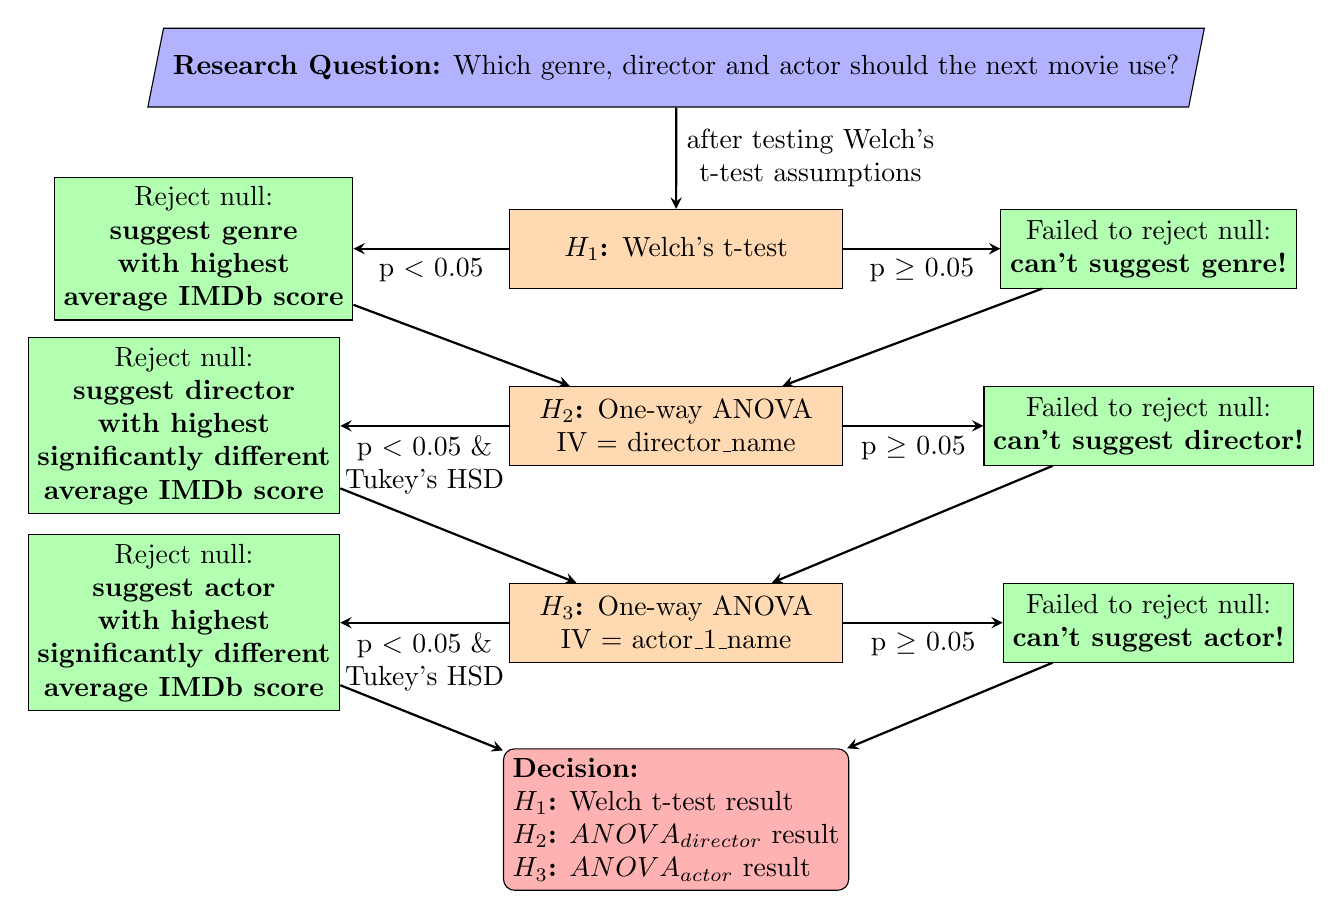
\begin{tikzpicture}[node distance=2cm]
\node (hyp1) [io, align=center] {\textbf{Research Question:} Which genre, director and actor should the next movie use?};

\node (ttest_1) [process, below of=hyp1, yshift=-0.3cm, align=center] {\textbf{$H_{1}$:} Welch's t-test};

\node (h0_1) [decision, left of=ttest_1, xshift=-4cm, align=center] {Reject null: \\ \textbf{suggest genre} \\ \textbf{with highest} \\ \textbf{average IMDb score}};

\node (ha_1) [decision, right of=ttest_1, xshift=4cm, align=center] {Failed to reject null: \\ \textbf{can't suggest genre!}};

\node (director) [process, below of=ttest_1, yshift=-0.25cm, align=center] {\textbf{$H_{2}$:} One-way ANOVA \\ IV = director\_name};

\node (h0_2) [decision, left of=director, xshift=-4.25cm, align=center] {Reject null: \\ \textbf{suggest director} \\ \textbf{with highest} \\ \textbf{significantly different} \\ \textbf{average IMDb score}};

\node (ha_2) [decision, right of=director, xshift=4cm, align=center] {Failed to reject null: \\ \textbf{can't suggest director!}};

\node (actor) [process, below of=director, yshift=-0.5cm, align=center] {\textbf{$H_{3}$:} One-way ANOVA \\ IV = actor\_1\_name};

\node (h0_3) [decision, left of=actor, xshift=-4.25cm, align=center] {Reject null: \\ \textbf{suggest actor} \\ \textbf{with highest} \\ \textbf{significantly different} \\ \textbf{average IMDb score}};

\node (ha_3) [decision, right of=actor, xshift=4cm, align=center] {Failed to reject null: \\ \textbf{can't suggest actor!}};

\node (out1) [startstop, below of=actor, align=left, yshift=-0.5cm] {\textbf{Decision:} \\\textbf{$H_{1}$:} Welch t-test result \\\textbf{$H_{2}$:} $ANOVA_{director}$ result \\ \textbf{$H_{3}$:} $ANOVA_{actor}$ result};

\draw [arrow] (hyp1) -- node[anchor=west, align=center] {after testing Welch's \\ t-test assumptions} (ttest_1);
\draw [arrow] (ttest_1) -- node[anchor=north] {p $<$ 0.05} (h0_1);
\draw [arrow] (ttest_1) -- node[anchor=north] {p $\ge$ 0.05} (ha_1);
\draw [arrow] (ha_1) -- (director);
\draw [arrow] (h0_1) -- (director);
\draw [arrow] (director) -- node[anchor=north, align=center] {p $<$ 0.05 \& \\ Tukey's HSD} (h0_2);
\draw [arrow] (director) -- node[anchor=north] {p $\ge$ 0.05} (ha_2);
\draw [arrow] (ha_2) -- (actor);
\draw [arrow] (h0_2) -- (actor);
\draw [arrow] (actor) -- node[anchor=north, align=center] {p $<$ 0.05 \& \\ Tukey's HSD} (h0_3);
\draw [arrow] (actor) -- node[anchor=north] {p $\ge$ 0.05} (ha_3);
\draw [arrow] (ha_3) -- (out1);
\draw [arrow] (h0_3) -- (out1);
\end{tikzpicture}
\end{center}

\pagebreak

\subsection{Data Cleaning \& EDA}

\subsubsection{Duplicates}

\emph{movie\_title}, \emph{title\_year}, and \emph{director\_name} were used to uniquely identify movies. Upon grouping by these features, 124 duplicate rows were removed.

\subsubsection{"Non-movies"}

Rows referring to "non-movies" (e.g., TV shows), aren’t relevant to this analysis and should be removed. Since every movie has a director, inspecting the data shows known "non-movie" rows do not (e.g., index-459: Daredevil). Removing these drops 102 rows.

\subsubsection{"Very Low" Review Count}

Too few reviews means sample IMDb scores are unreliable estimates; data inspection could help define “too few”.

\begin{center}
    \captionof{figure}{Distribution of Number of Unique Reviewers for Each Movie}
    \includegraphics[scale = 0.7]{review_hist.png}
\end{center}

\pagebreak
\begin{center}
    \captionof{figure}{\emph{Logarithmic} Distributions of Number of Unique Reviewers for Each Movie}
    \includegraphics[scale = 0.55]{review_hist_log.png}
\end{center}

\textbf{Figure 2} shows an approximate log-normal distribution, thus removing values where $x < 3\sigma$ is inappropriate $(i.e.~\bar{x}-\sigma = -55,658.79)$. For \emph{num\_voted\_users}, converting to a logarithmic x-axis shows the negative skew (\textbf{Figure 3}) is mainly due to reviews $\lessapprox 1000$. Thus 364 rows with $\lessapprox 1000$ reviews were removed.

\subsubsection{Missing data}

Missing data in key features is problematic. Examining missing values in romance and horror movies (removing 17 romance-horror rows) and comparing them to the overall dataset avoids inadvertently removing these genres if they happened to contribute disproportionately to missing data.

\begin{center}
\captionof{table}{Top 5 Columns with the Most Nulls (Entire Dataset).}
\begin{tabular}{lrr}
\toprule
Column Name & Nulls & Percentage of Total Rows \\
\midrule
gross & 508 & 11.4 \\
budget & 306 & 6.9 \\
aspect\_ratio & 115 & 2.6 \\
content\_rating & 106 & 2.4 \\
plot\_keywords & 32 & 0.7 \\
\bottomrule
\end{tabular}
\vspace*{5mm}
\captionof{table}{Top 5 Columns with the Most Nulls (Horror Subset, N = 474).}
\begin{tabular}{lrr}
\toprule
Column Name & Nulls & Percentage of Total Rows \\
\midrule
gross & 97 & 20.5 \\
budget & 24 & 5.1 \\
aspect\_ratio & 14 & 3.0 \\
content\_rating & 11 & 2.3 \\
plot\_keywords & 2 & 0.4 \\
\bottomrule
\end{tabular}
\vspace*{10mm}
\captionof{table}{Top 5 Columns with the Most Nulls (Romance Subset, N = 1002).}
\begin{tabular}{lrr}
\toprule
Column Name & Nulls & Percentage of Total Rows \\
\midrule
gross & 97 & 9.7 \\
budget & 71 & 7.1 \\
content\_rating & 24 & 2.4 \\
aspect\_ratio & 19 & 1.9 \\
plot\_keywords & 5 & 0.5 \\
\bottomrule
\end{tabular}
\end{center}

\textbf{Table 3 \& 4} show subsets aren’t disproportionately representative of nulls. Removing them will not omit our target genres. \textit{gross} and \textit{budget} are our measure of profit when assessing the IMDb-profit assumption, so we’ll remove null rows from these columns. Doing so drops 263.

\subsubsection{Assessing IMDb-profit Assumption}

Creating a \textit{profit} column (\textit{gross} minus \textit{budget}) and correlating it with \textit{imdb\_score}:

\begin{center}
    \captionof{figure}{}
    \includegraphics[scale = 0.585]{corr_df}
\end{center}

\pagebreak
A near-zero correlation $r(3609) = .03,~p < .05$. The lowest data point in Figure 4 shows the budget is in native currency $(budget = 12,215,500,000,~gross = 2,201,412)$, not USD. Furthermore, \textit{gross} and \textit{budget} aren’t inflation-adjusted. After removing 778 non-US movies and adjusting values to 2023 USD using CPI data (Bureau of Labor Statistics, 2024), the correlation becomes stronger but still weak at 0.26, limiting conclusions.

\begin{center}
    \captionof{figure}{}
    \includegraphics[scale = 0.585]{corr_df_usa}
\end{center}

\subsubsection{Older Movies}

I kept all release years since IMDb scores are consistent over time for both genres:

\begin{center}
    \captionof{figure}{Scatter Plot Comparing IMDb Score Trends Over Time for Romance (red) and Horror (green) Movies}
    \includegraphics[scale = 0.525]{trend}
\end{center}

\subsection{Summary}

42\% of the data was removed, reducing from 5,043 to 2,918. This limits the analysis to the US market but greatly improves reliability.

\pagebreak
\section{Results}

\subsection{Top 10 Highest Rated Movies}

\textbf{Table 5} shows the top 10 highest-rated movies, ranked first by IMDb score, then by review count.

\begin{center}
\captionof{table}{Top 10 Movies with the Highest IMDb Ratings.}
\begin{tabular}{p{0.75cm}p{5cm}ccc}
\toprule
Rank & Movie Title & Year Released & IMDb Score & Number of User Reviews \\
\midrule
1st & The Shawshank Redemption  & 1994 & 9.3 & 1,689,764 \\
2nd & The Godfather  & 1972 & 9.2 & 1,155,770 \\
3rd & The Dark Knight  & 2008 & 9.0 & 1,676,169 \\
4th & The Godfather: Part II  & 1974 & 9.0 & 790,926 \\
5th & Pulp Fiction  & 1994 & 8.9 & 1,324,680 \\
6th & The Lord of the Rings: The Return of the King  & 2003 & 8.9 & 1,215,718 \\
7th & Schindler's List  & 1993 & 8.9 & 865,020 \\
8th & The Good, the Bad and the Ugly  & 1966 & 8.9 & 503,509 \\
9th & 12 Angry Men  & 1957 & 8.9 & 447,785 \\
10th & Inception  & 2010 & 8.8 & 1,468,200 \\
\bottomrule
\end{tabular}

\begin{tablenotes}
    \centering
    \small
    \item \textbf{Note:} Based on Movies with $N > 1000$ User Reviews, including non-US movies
\end{tablenotes}
\end{center}

\subsection{Top 5 Most Common Genres}

\textbf{Table 6} shows the top 5 genres by movie count, supported by \textbf{Figure 7} showing IMDb score distributions and summary statistics.

\begin{center}
\captionof{table}{Top 5 Individual Genres with the Most Number of Movies.}
\begin{tabular}{p{5cm}c}
\toprule
Genre & Number of Movies \\
\midrule
Drama & 2,290 \\
Comedy & 1,725 \\
Thriller & 1,269 \\
Action & 1,046 \\
Romance & 1,019 \\
\bottomrule
\end{tabular}

\begin{tablenotes}
    \centering
    \small
    \item \textbf{Note:} Based on Movies with $N > 1000$ User Reviews, including non-US movies
\end{tablenotes}
\end{center}

\pagebreak
\begin{center}
    \captionof{figure}{Histograms Displaying the Distribution of IMDb Scores for Each of the Top 5 Genres with the Most Movies, Along with Summary Statistics for Each Plot.}
    \vspace*{-0.375cm}
    \includegraphics[scale = 0.55]{top5histplots}
\end{center}

\pagebreak
\subsection{Romance vs Horror: Two-Tailed Welch's t-test}

Given the IMDb distributions are approximately Gaussian:

\begin{center}
    \captionof{figure}{P-P Plot Comparing the Empirical Cumulative Distribution Functions of Romance (red) and Horror (green) Movie IMDb Scores to a Theoretical Gaussian CDF}
    \includegraphics[scale = 0.65]{ppplot}
\end{center}

Welch’s t-test shows a significant difference between IMDb scores for \emph{romance} $(\bar{x} = 6.35,~\sigma = 0.95,~N = 663)$ and \emph{horror} $(\bar{x} = 5.87,~\sigma = 0.98,~N = 291)$ movies, $t(537.40) = 7.03,~p < .05,~95\%~CI~[0.346,~0.614]$. Rejecting the null hypothesis, \emph{romance} movies have a significantly higher average IMDb.

\begin{center}
    \captionof{figure}{KDE Plot Comparing IMDb Score Distributions of Romance (red) and Horror (green) Movies}
    \includegraphics[scale = 0.75]{Hyp1_KDE}
\end{center}

\pagebreak
\subsection{Choosing a Director}

\subsubsection{Two-tailed One-way ANOVA}

ANOVA found at least 1 mean was significantly different $F(125, 199) = 1.89,~p < 0.05$, thus the null hypothesis is rejected.

\subsubsection{Tukey's HSD}

\begin{center}
    \captionof{figure}{Mean Plot Comparing Average IMDb Scores of Directors Found to be Significantly Different by Tukey's HSD}
    \includegraphics[scale = 0.5]{director_tukey}
\end{center}

No director "dominates," but there's a bifurcation (red line) into "higher" and "lower" IMDb averages. The error bars show \textit{Richard Linklater}, \textit{Stephen Daldry} and \textit{Tim Burton} have significantly higher averages than the "lower" group (green line). Given \textit{Linklater} has the highest, they are the recommended director.

\pagebreak
\subsection{Choosing a Lead Actor}

\subsubsection{Two-tailed One-way ANOVA}

ANOVA found at least 1 mean was significantly different $F(116, 246) = 1.81,~p < 0.05$, thus the null hypothesis is rejected.

\subsubsection{Tukey's HSD}

\begin{center}
    \captionof{figure}{Mean Plot Comparing Average IMDb Scores of Actors Found to be Significantly Different by Tukey's HSD}
    \includegraphics[scale = 0.5]{actor_tukey}
\end{center}

Whilst \textit{Kate Winslet} and \textit{Ryan Gosling} have the highest average IMDbs, there is little to separate them. Given \textit{Winslet's} average is slightly higher $(\bar{x} = 7.600)$ than \textit{Gosling's} $(\bar{x} = 7.525)$, \textit{Winslet} is the recommended actor.

\pagebreak
\section{Conclusion}

\begin{center}
\captionof{table}{Recommendations from the Analysis}
\begin{tabular}{p{3cm}p{3cm}}
 & \\
Genre: & Romance \\
Director: & Richard Linklater \\
Lead Actor: & Kate Winslet \\

\end{tabular}
\begin{tablenotes}
    \centering
    \small
    \item
    \item \textit{\textbf{Note:} This table was produced in the PDF's .tex file, not the .py script}
\end{tablenotes}
\end{center}

To conclude, with a cleaned sample of 2,918 US movies, a two-tailed Welch's t-test revealed \textit{romance} movies - the recommended genre - have a significantly higher average IMDb score compared to \textit{horror} movies. Furthermore, two-tailed one-way ANOVAs, followed by post-hoc Tukey HSDs provided \textit{Richard Linklater} as recommended director, with \textit{Kate Winslet} as recommended lead. 

Such a triplet of suggestions is a best estimate for maximising profit from the next movie, with the following limitations kept in mind:

\begin{enumerate}
    \item Conclusions only apply to the US market.
    \item IMDb score shares a weak positive correlation with profit, and an undetermined causal relation.
    \item Director/actor selection post Tukey's HSD arguably lacks statistical justification.
    \item Only directors and actors who have previously appeared in romance movies were considered (since they have relevant data that can be analysed) - non-romance directors/actors may still outperform those recommended. 
\end{enumerate}

\pagebreak
\section{References}

Bureau of Labor Statistics Data. (2024). Bureau of Labor Statistics. https://data.bls.gov/timeseries/CUUR0000SA0

IMDb: Ratings, Reviews, and Where to Watch the Best Movies \& TV Shows. (2024). IMDb. https://www.imdb.com/

\end{document}